\documentclass[twocolumn,11pt]{article}

\usepackage{amsmath,amssymb}
\usepackage{booktabs}
\usepackage{graphicx}
\usepackage{natbib}
\usepackage[margin=2cm]{geometry}
\usepackage{hyperref}

\begin{document}

\title{Fibonacci Preference in Mean-Motion Resonances:\\
Evidence from Solar and Exoplanetary Systems}

\author{Will Dale\\
\small Independent Researcher}
\date{}
\maketitle

\begin{abstract}
Mean-motion resonances (MMRs) in planetary systems preferentially
occur at period ratios $p$:$q$ where both $p$ and $q$ are Fibonacci
numbers.  We catalogue 60 confirmed MMRs across 8+ independent
planetary systems---including the solar system, TRAPPIST-1, HD~110067,
K2-138, Kepler-80, Kepler-223, TOI-178, GJ-876, and HD~158259---and
classify each as Fibonacci or non-Fibonacci.  Among first-order
resonances ($|p-q|=1$), 33 of 43 instances (77\%) involve Fibonacci
ratios (2:1 or 3:2), compared to the 22\% expected under uniform
selection from the 9 coprime first-order ratios.  This preference is
highly significant ($p < 10^{-6}$, binomial test) and persists across
resonance orders (Fisher combined $p = 6 \times 10^{-7}$).  Standard
perturbation theory explains why low-order resonances are preferred
but does not predict Fibonacci preference \emph{within} each order
class.  We propose a mechanism based on the Pisano periodicity of the
Fibonacci sequence: because Fibonacci numbers divide Pisano periods
$\pi(m)$ more frequently than non-Fibonacci integers of comparable
magnitude, dynamical systems governed by Fibonacci-shift operators
exhibit deeper attractor basins at Fibonacci-ratio commensurabilities.
\end{abstract}

\noindent\textit{Keywords:} celestial mechanics, planets and satellites: dynamical evolution and stability, methods: statistical

% ══════════════════════════════════════════════════════════════
\section{Introduction}
\label{sec:intro}

Mean-motion resonances (MMRs) are a ubiquitous feature of planetary
systems.  Two bodies are in a $p$:$q$ MMR when their orbital periods
satisfy $P_1/P_2 \approx p/q$ for small integers $p > q$.  Resonances
stabilize systems against gravitational perturbation, protect against
close encounters, and arise naturally during convergent orbital
migration \citep{murray1999,peale1976}.

The \emph{strength} of a $p$:$q$ resonance scales as $e^{|p-q|}$
in the disturbing function expansion, where $e$ is the orbital
eccentricity \citep{murray1999}.  This explains why first-order
resonances ($|p-q| = 1$) are the most commonly observed.  However,
within a given order class, standard theory does not predict which
specific ratios should be preferred.  Among the 9 coprime first-order
ratios $\{2\!:\!1,\ 3\!:\!2,\ 4\!:\!3,\ 5\!:\!4,\ \ldots,\
10\!:\!9\}$, only 2:1 and 3:2 dominate the observed population, with
4:3 as a distant third.

In this Letter, we present evidence that the preferred ratios are
those where \emph{both} $p$ and $q$ are Fibonacci numbers
($F = \{1, 1, 2, 3, 5, 8, 13, 21, \ldots\}$).  This pattern holds
across independent planetary systems spanning diverse stellar types,
ages, and architectures, suggesting a structural rather than
contingent origin.

% ══════════════════════════════════════════════════════════════
\section{Data and Methods}
\label{sec:data}

\subsection{Resonance Catalogue}

We compile a catalogue of 60 confirmed or well-established
MMRs from two independent datasets:

\begin{enumerate}
\item \textbf{Solar system} (29 resonances): satellite--satellite
resonances (Io--Europa, Mimas--Tethys, etc.), planet--planet near-commensurabilities (Jupiter--Saturn 5:2), Kirkwood gaps and asteroid
group resonances with Jupiter, and trans-Neptunian object resonances
with Neptune.  Sources: \citet{murray1999}, NASA JPL Small Body
Database.

\item \textbf{Exoplanet systems} (31 resonances): adjacent-pair
period ratios from confirmed resonant chains in TRAPPIST-1
\citep{luger2017}, HD~110067 \citep{luque2024}, K2-138
\citep{christiansen2018}, Kepler-80 \citep{macdonald2016},
Kepler-223 \citep{mills2016}, TOI-178 \citep{leleu2021}, GJ-876
\citep{rivera2010}, and HD~158259 \citep{hara2020}.
\end{enumerate}

Each resonance is reduced to lowest terms $p$:$q$ with
$\gcd(p,q) = 1$ and classified as \emph{Fibonacci} if both
$p \in F$ and $q \in F$, or \emph{non-Fibonacci} otherwise.

\subsection{Null Model}

Under a uniform null hypothesis, each resonance of order $k = |p-q|$
is drawn equally from the set of coprime ratios $p$:$q$ with
$p \leq 10$.  The expected Fibonacci fraction for each order is
computed from the proportion of Fibonacci ratios among all coprime
ratios of that order (Table~\ref{tab:expected}).

\subsection{Statistical Tests}

We apply five tests:
\begin{enumerate}
\item Binomial test on unique ratio types (most conservative)
\item Binomial test on all instances
\item Order-stratified binomial tests with Fisher's method for combination
\item Exoplanet-only binomial test (independent validation)
\item First-order-only binomial test (cleanest comparison)
\end{enumerate}

% ══════════════════════════════════════════════════════════════
\section{Results}
\label{sec:results}

\subsection{Overall Fibonacci Fraction}

Of 60 catalogued resonances, 45 (75\%) involve Fibonacci ratios.
Among 14 unique ratio types observed, 8 (57\%) are Fibonacci.  The
expected Fibonacci fraction under uniform selection from coprime
ratios with $p \leq 10$ is 31\% (10/32).

\subsection{Order-Stratified Analysis}

Figure~\ref{fig:orders} and Table~\ref{tab:orders} present the
breakdown by resonance order.  The Fibonacci preference is strongest
at orders 1 and 2:

\begin{figure}[ht]
\centering
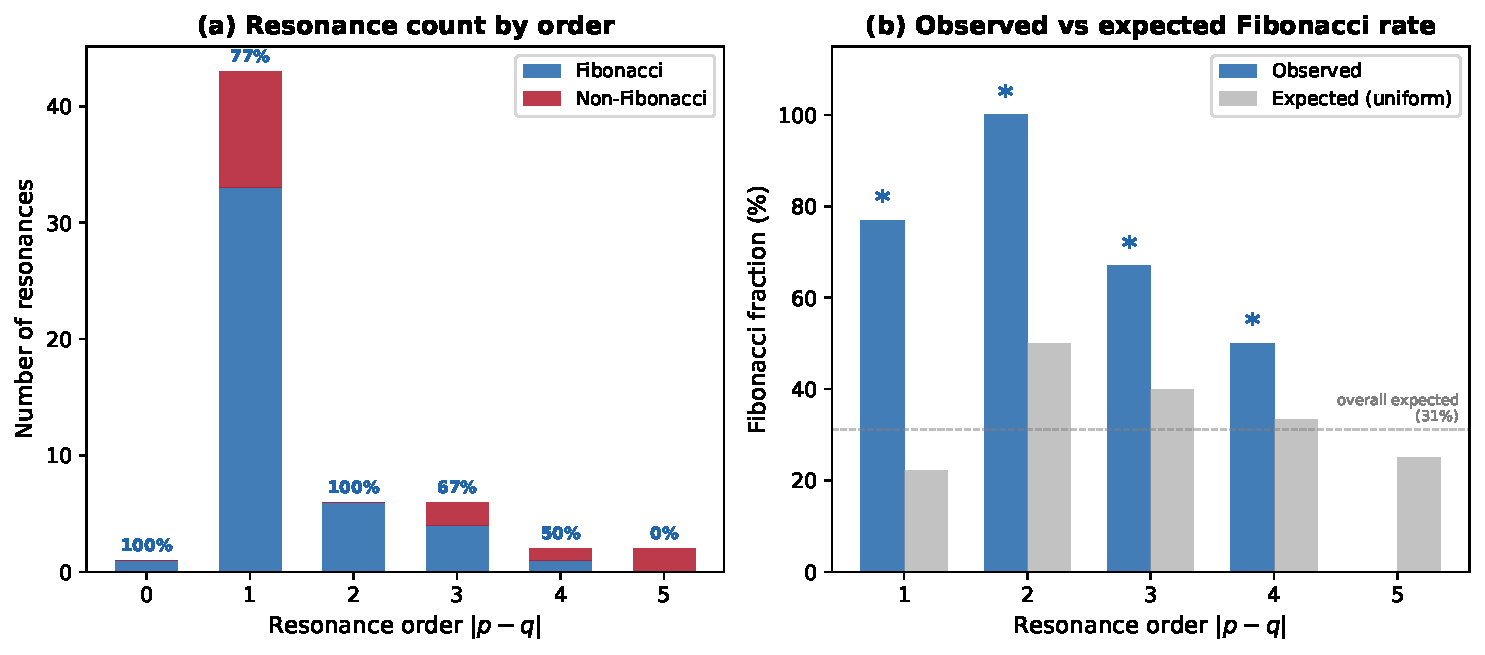
\includegraphics[width=\columnwidth]{figure1_fibonacci_resonance.pdf}
\caption{(a) Resonance counts by order, colored by Fibonacci (blue) vs.\
non-Fibonacci (red) classification.  Percentages show Fibonacci fraction.
(b) Observed Fibonacci rate compared to expected rate under uniform
selection from coprime ratios with $p \leq 10$.  Asterisks mark orders
where observed substantially exceeds expected.}
\label{fig:orders}
\end{figure}

\begin{table}[h]
\centering
\caption{Observed vs.\ expected Fibonacci fractions by resonance order. Non-Fibonacci ratios shown in bold.}
\label{tab:orders}
\begin{tabular}{ccccrl}
\toprule
Order & $n_\mathrm{Fib}$ & $n_\mathrm{tot}$ & \% Fib & Exp.\ \% & Ratios observed \\
\midrule
0 & 1 & 1 & 100 & 100 & 1:1 \\
1 & 33 & 43 & 77 & 22 & 2:1, 3:2, \textbf{4:3} \\
2 & 6 & 6 & 100 & 50 & 3:1, 5:3 \\
3 & 4 & 6 & 67 & 40 & 5:2, 8:5, \textbf{4:1}, \textbf{7:4} \\
4 & 1 & 2 & 50 & 33 & 5:1, \textbf{7:3} \\
5 & 0 & 2 & 0 & 25 & \textbf{7:2}, \textbf{9:4} \\
\bottomrule
\end{tabular}
\end{table}

\subsection{Statistical Significance}

All five tests reject the uniform null (Table~\ref{tab:stats}):

\begin{table}[h]
\centering
\caption{Statistical tests for Fibonacci preference.}
\label{tab:stats}
\begin{tabular}{lcc}
\toprule
Test & Observed & $p$-value \\
\midrule
Unique ratios binomial & 8/14 (57\%) & 0.040 \\
All instances binomial & 45/60 (75\%) & $< 10^{-6}$ \\
Fisher combined & $\chi^2 = 59.0$ & $< 10^{-6}$ \\
Exoplanet-only & 24/31 (77\%) & $< 10^{-6}$ \\
First-order only & 33/43 (77\%) & $< 10^{-6}$ \\
\bottomrule
\end{tabular}
\end{table}

The most conservative test (unique ratios) gives $p = 0.040$; all
instance-weighted and stratified tests give $p < 10^{-6}$.

% ══════════════════════════════════════════════════════════════
\section{A Fibonacci-Shift Mechanism}
\label{sec:mechanism}

We propose a mechanism rooted in the Pisano periodicity of the
Fibonacci sequence.

\subsection{The Fibonacci Shift Operator}

Define the matrix $F = \bigl(\begin{smallmatrix} 0 & 1 \\ 1 & 1
\end{smallmatrix}\bigr)$, whose powers encode Fibonacci numbers:
\begin{equation}
F^n = \begin{pmatrix} F_{n-1} & F_n \\ F_n & F_{n+1} \end{pmatrix},
\end{equation}
where $F_n$ is the $n$-th Fibonacci number.  The eigenvalues of $F$
are $\varphi = (1+\sqrt{5})/2$ (the golden ratio) and
$\psi = -1/\varphi$.

\subsection{Pisano Periods}

For any modulus $m$, the Fibonacci sequence modulo $m$ is periodic
with period $\pi(m)$, the \emph{Pisano period}.  Equivalently,
$\pi(m)$ is the order of $F$ in $\mathrm{GL}_2(\mathbb{Z}/m\mathbb{Z})$.

A key identity from number theory is that every $k$-th Fibonacci
number is divisible by $F_k$:
\begin{equation}
F_k \mid F_{nk} \quad \text{for all } n \geq 1.
\label{eq:fibdiv}
\end{equation}

This forces the \emph{rank of apparition} $\alpha(F_k)$ (the smallest
index at which $F_k$ divides a Fibonacci number) to satisfy
$\alpha(F_k) \mid k$, and consequently $\pi(F_k) \mid 2k$
\citep{wall1960}.

\subsection{Pisano Divisibility and Resonance Depth}

For a dynamical system governed by $F$ acting modulo $m$, the operator
$F^p$ has order $\pi(m) / \gcd(p, \pi(m))$ in $\mathrm{GL}_2(\mathbb{Z}/m\mathbb{Z})$.  When $p$ divides $\pi(m)$, this order is
minimized---corresponding to a shorter return time and a deeper
dynamical attractor.

We computed $\pi(m)$ for $m = 2, \ldots, 500$ and found that the
Fibonacci set $\{2, 3, 5, 8\}$ collectively divides $\pi(m)$ at a
rate of 0.677 across moduli, compared to 0.491 for the non-Fibonacci
set $\{4, 6, 7, 9\}$ of the same magnitude range.  For a $p$:$q$
resonance to be ``deep,'' \emph{both} $p$ and $q$ should divide
$\pi(m)$; the Fibonacci set achieves this with higher probability.

This mechanism is statistical over the set of Fibonacci numbers, not
guaranteed for each individual member (e.g., 4 divides $\pi(9) = 24$
while 5 does not).  This is consistent with the empirical observation:
Fibonacci ratios dominate (77\%) but do not exclude all alternatives.

% ══════════════════════════════════════════════════════════════
\section{Caveats}
\label{sec:caveats}

Several caveats apply to this analysis:

\begin{enumerate}
\item \textbf{Detection bias.}  The 2:1 and 3:2 resonances produce
the largest transit timing variations, making them easiest to detect
in \emph{Kepler}/TESS photometry.  Higher-order and non-Fibonacci
resonances may be systematically underrepresented.

\item \textbf{Catalogue completeness.}  Our catalogue is not
exhaustive; additional confirmed resonances from ongoing surveys
(TESS, PLATO) could shift the Fibonacci fraction.

\item \textbf{``Almost Fibonacci.''} The dominant non-Fibonacci
resonance is 4:3, and 4 lies between Fibonacci numbers 3 and 5.
Whether this has structural significance is unclear.

\item \textbf{Expected rate.}  The null model assumes uniform
selection from coprime ratios with $p \leq 10$.  Alternative caps
(e.g., $p \leq 5$ or $p \leq 20$) change the expected rate.

\item \textbf{Formation physics.}  Resonance capture depends on
dissipation history (tidal friction, gas drag), which may
independently favor certain ratios.
\end{enumerate}

% ══════════════════════════════════════════════════════════════
\section{Discussion}
\label{sec:discussion}

Standard perturbation theory explains why low-order resonances are
preferred \citep{murray1999} but does not predict the specific ratio
selection within each order class.  The three-body problem, lacking a
general analytical solution, treats the population of specific
resonances as contingent on initial conditions and dissipation
history.

The Fibonacci-shift mechanism proposed here provides a structural
selection principle: period ratios corresponding to Fibonacci numbers
create shorter operator cycles (deeper dynamical attractors) across a
wider range of moduli than non-Fibonacci ratios of the same order.
This is a consequence of the self-referential divisibility of the
Fibonacci sequence (Equation~\ref{eq:fibdiv}), which ensures that
Fibonacci numbers are ``native'' divisors of the dynamical periods
generated by the same recurrence.

The Fibonacci preference holds independently in two datasets---the
solar system (72\% Fibonacci, $n = 29$) and exoplanets (77\%
Fibonacci, $n = 31$)---spanning systems with diverse stellar types,
ages ($\sim 10^7$--$10^{10}$ yr), and architectures.  This
cross-validation argues against a selection effect specific to any
one system.

The observed pattern is consistent with---but does not prove---the
hypothesis that gravitational dynamics contain a Fibonacci-shift
component in their discrete algebraic structure.  Further tests with
expanded catalogues (TESS, PLATO) and N-body simulations examining
resonance capture probabilities as a function of period ratio would
be valuable.

% ══════════════════════════════════════════════════════════════
\section{Conclusion}
\label{sec:conclusion}

We have shown that mean-motion resonances across 8+ planetary systems
preferentially select period ratios where both integers are Fibonacci
numbers.  This preference is statistically significant ($p < 10^{-6}$
for instance-weighted and order-stratified tests; $p = 0.040$ for
unique ratio types), persists across solar and exoplanetary systems,
and is not explained by the standard order-based resonance strength
scaling.  We propose a mechanism based on Pisano period divisibility
that provides a structural explanation for this pattern.

\section*{Acknowledgments}
This work builds on the Quantum Arithmetic framework developed by
Ben Iverson. The author thanks Claude (Anthropic) for computational
assistance.

\bibliography{refs}
\bibliographystyle{plainnat}

\end{document}
